\chapter{Supporting Material for Chapter 3, Results}
\label{cha:app3}
\begin{figure}
\centering
    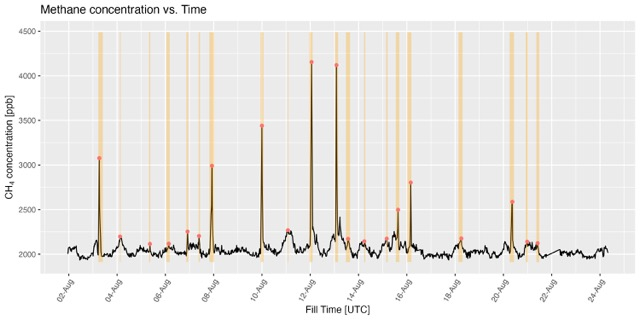
\includegraphics[width=.8\textwidth]{figures/Appendix/CH4_Timelines/MediumPeakTimeline/4_CH4_Timeline0_Medium_Peaks Medium.jpeg}
    \\[\smallskipamount]
    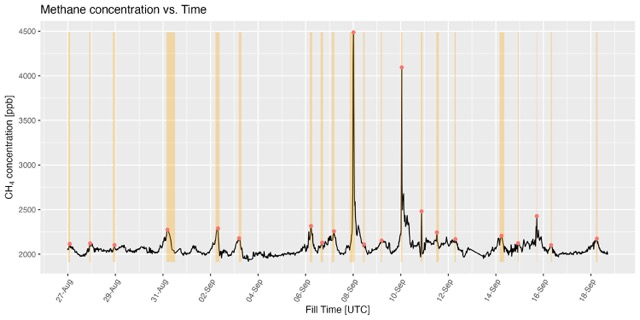
\includegraphics[width=.8\textwidth]{figures/Appendix/CH4_Timelines/MediumPeakTimeline/4_CH4_Timeline1_Medium_Peaks Medium.jpeg}
    \\[\smallskipamount]
    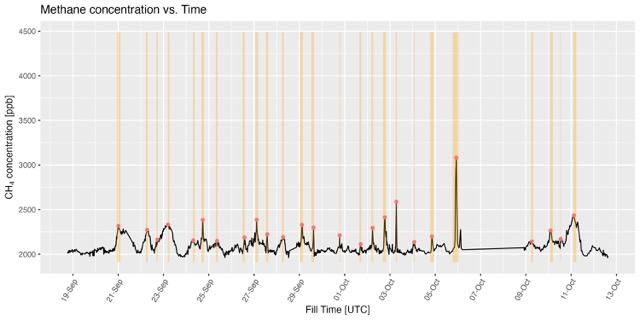
\includegraphics[width=.8\textwidth]{figures/Appendix/CH4_Timelines/MediumPeakTimeline/4_CH4_Timeline2_Medium_Peaks Medium.jpeg}
    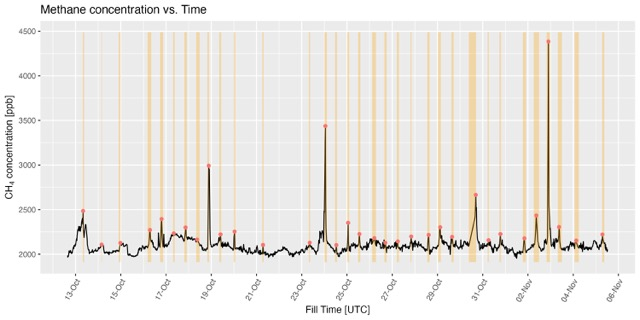
\includegraphics[width=.8\textwidth]{figures/Appendix/CH4_Timelines/MediumPeakTimeline/4_CH4_Timeline3_Medium_Peaks Medium.jpeg}
\end{figure}
\begin{figure} 
\centering
    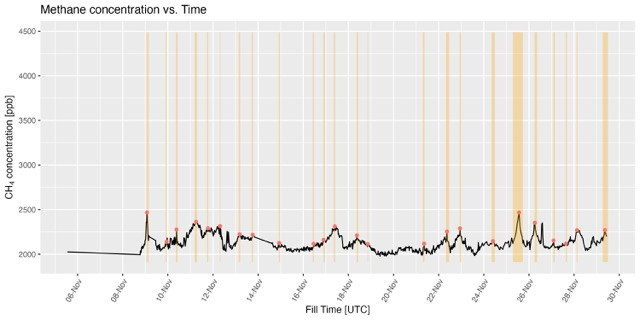
\includegraphics[width=.8\textwidth]{figures/Appendix/CH4_Timelines/MediumPeakTimeline/4_CH4_Timeline4_Medium_Peaks Medium.jpeg}
    \\[\smallskipamount]
    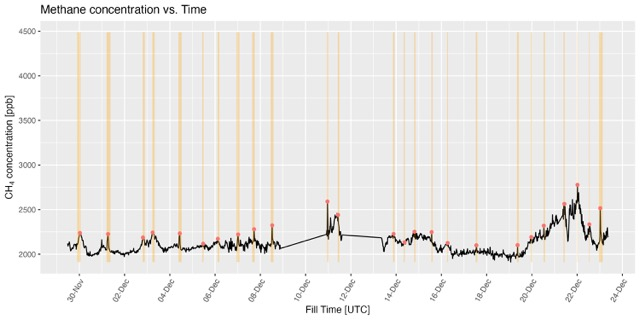
\includegraphics[width=.8\textwidth]{figures/Appendix/CH4_Timelines/MediumPeakTimeline/4_CH4_Timeline5_Medium_Peaks Medium.jpeg}
    \\[\smallskipamount]
    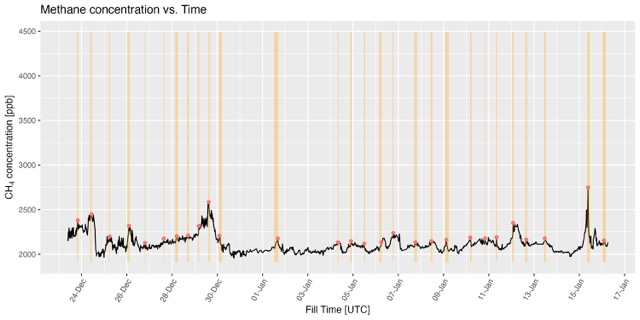
\includegraphics[width=.8\textwidth]{figures/Appendix/CH4_Timelines/MediumPeakTimeline/4_CH4_Timeline6_Medium_Peaks Medium.jpeg}
    \\[\smallskipamount]
    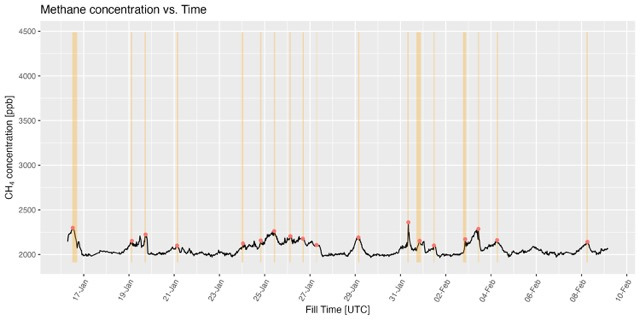
\includegraphics[width=.8\textwidth]{figures/Appendix/CH4_Timelines/MediumPeakTimeline/4_CH4_Timeline7_Medium_Peaks Medium.jpeg}
\end{figure}
\begin{figure}    
\centering
    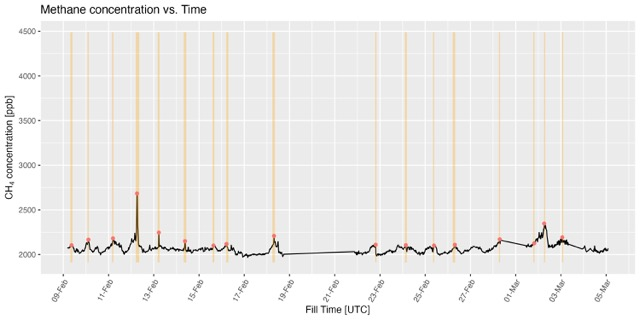
\includegraphics[width=.8\textwidth]{figures/Appendix/CH4_Timelines/MediumPeakTimeline/4_CH4_Timeline8_Medium_Peaks Medium.jpeg}
    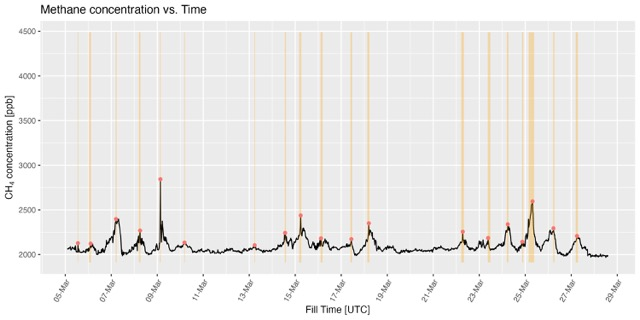
\includegraphics[width=.8\textwidth]{figures/Appendix/CH4_Timelines/MediumPeakTimeline/4_CH4_Timeline9_Medium_Peaks Medium.jpeg}
    \caption[Complete CF-IRMS time-line with prominent peaks highlighted]{Complete CF-IRMS measurement time-line, measured at the Geomatikum at an altitude of 83m above street level. Measurements from  02.08.2021 to 29.03.2021 are shown. Prominent peaks are identified and highlighted. Red dot for peak centre and orange highlight box for peak width.}
    \label{CompleteCF-IRMSTimeinePeaksAppendix}
\end{figure}

\begin{figure}[!htb]
\centering
\begin{subfigure}[b]{0.8\textwidth}
   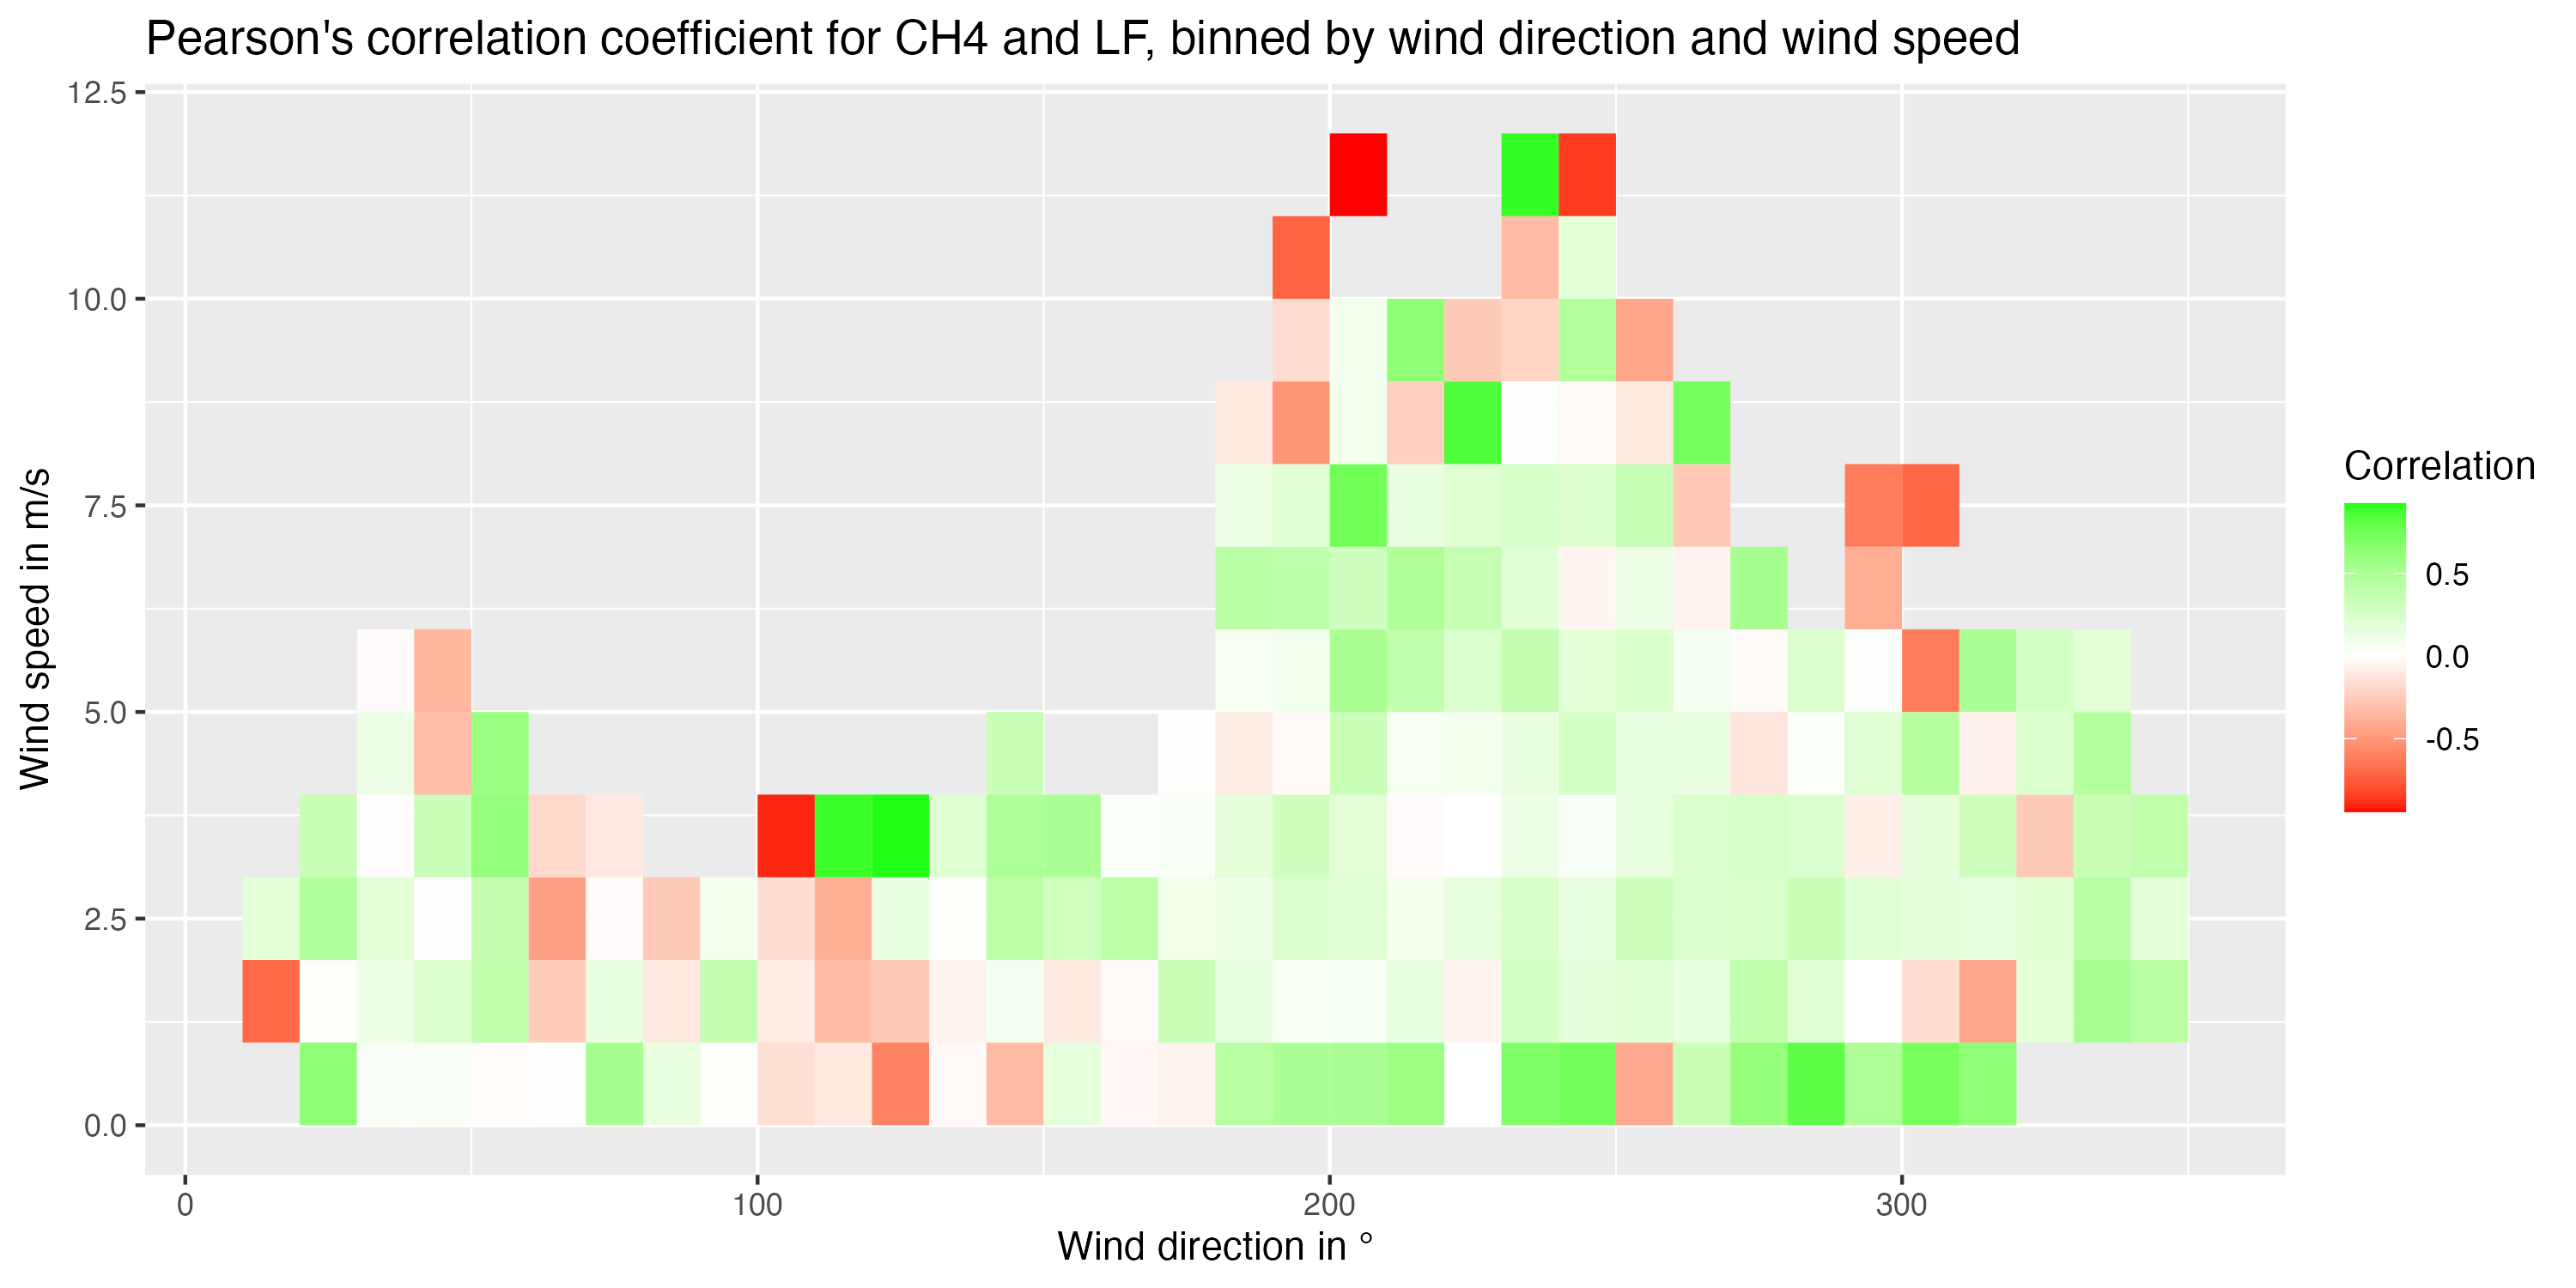
\includegraphics[width=1\linewidth]{figures/Appendix/NoCorrelation/13_CH4_vs_Conductivity_Correlation_Geomatikum.png}
   \caption[NCorrelation plot conductivity in Elbe water]{}
   \label{NoCorrelationConductivity} 
\end{subfigure}
\begin{subfigure}[b]{0.8\textwidth}
   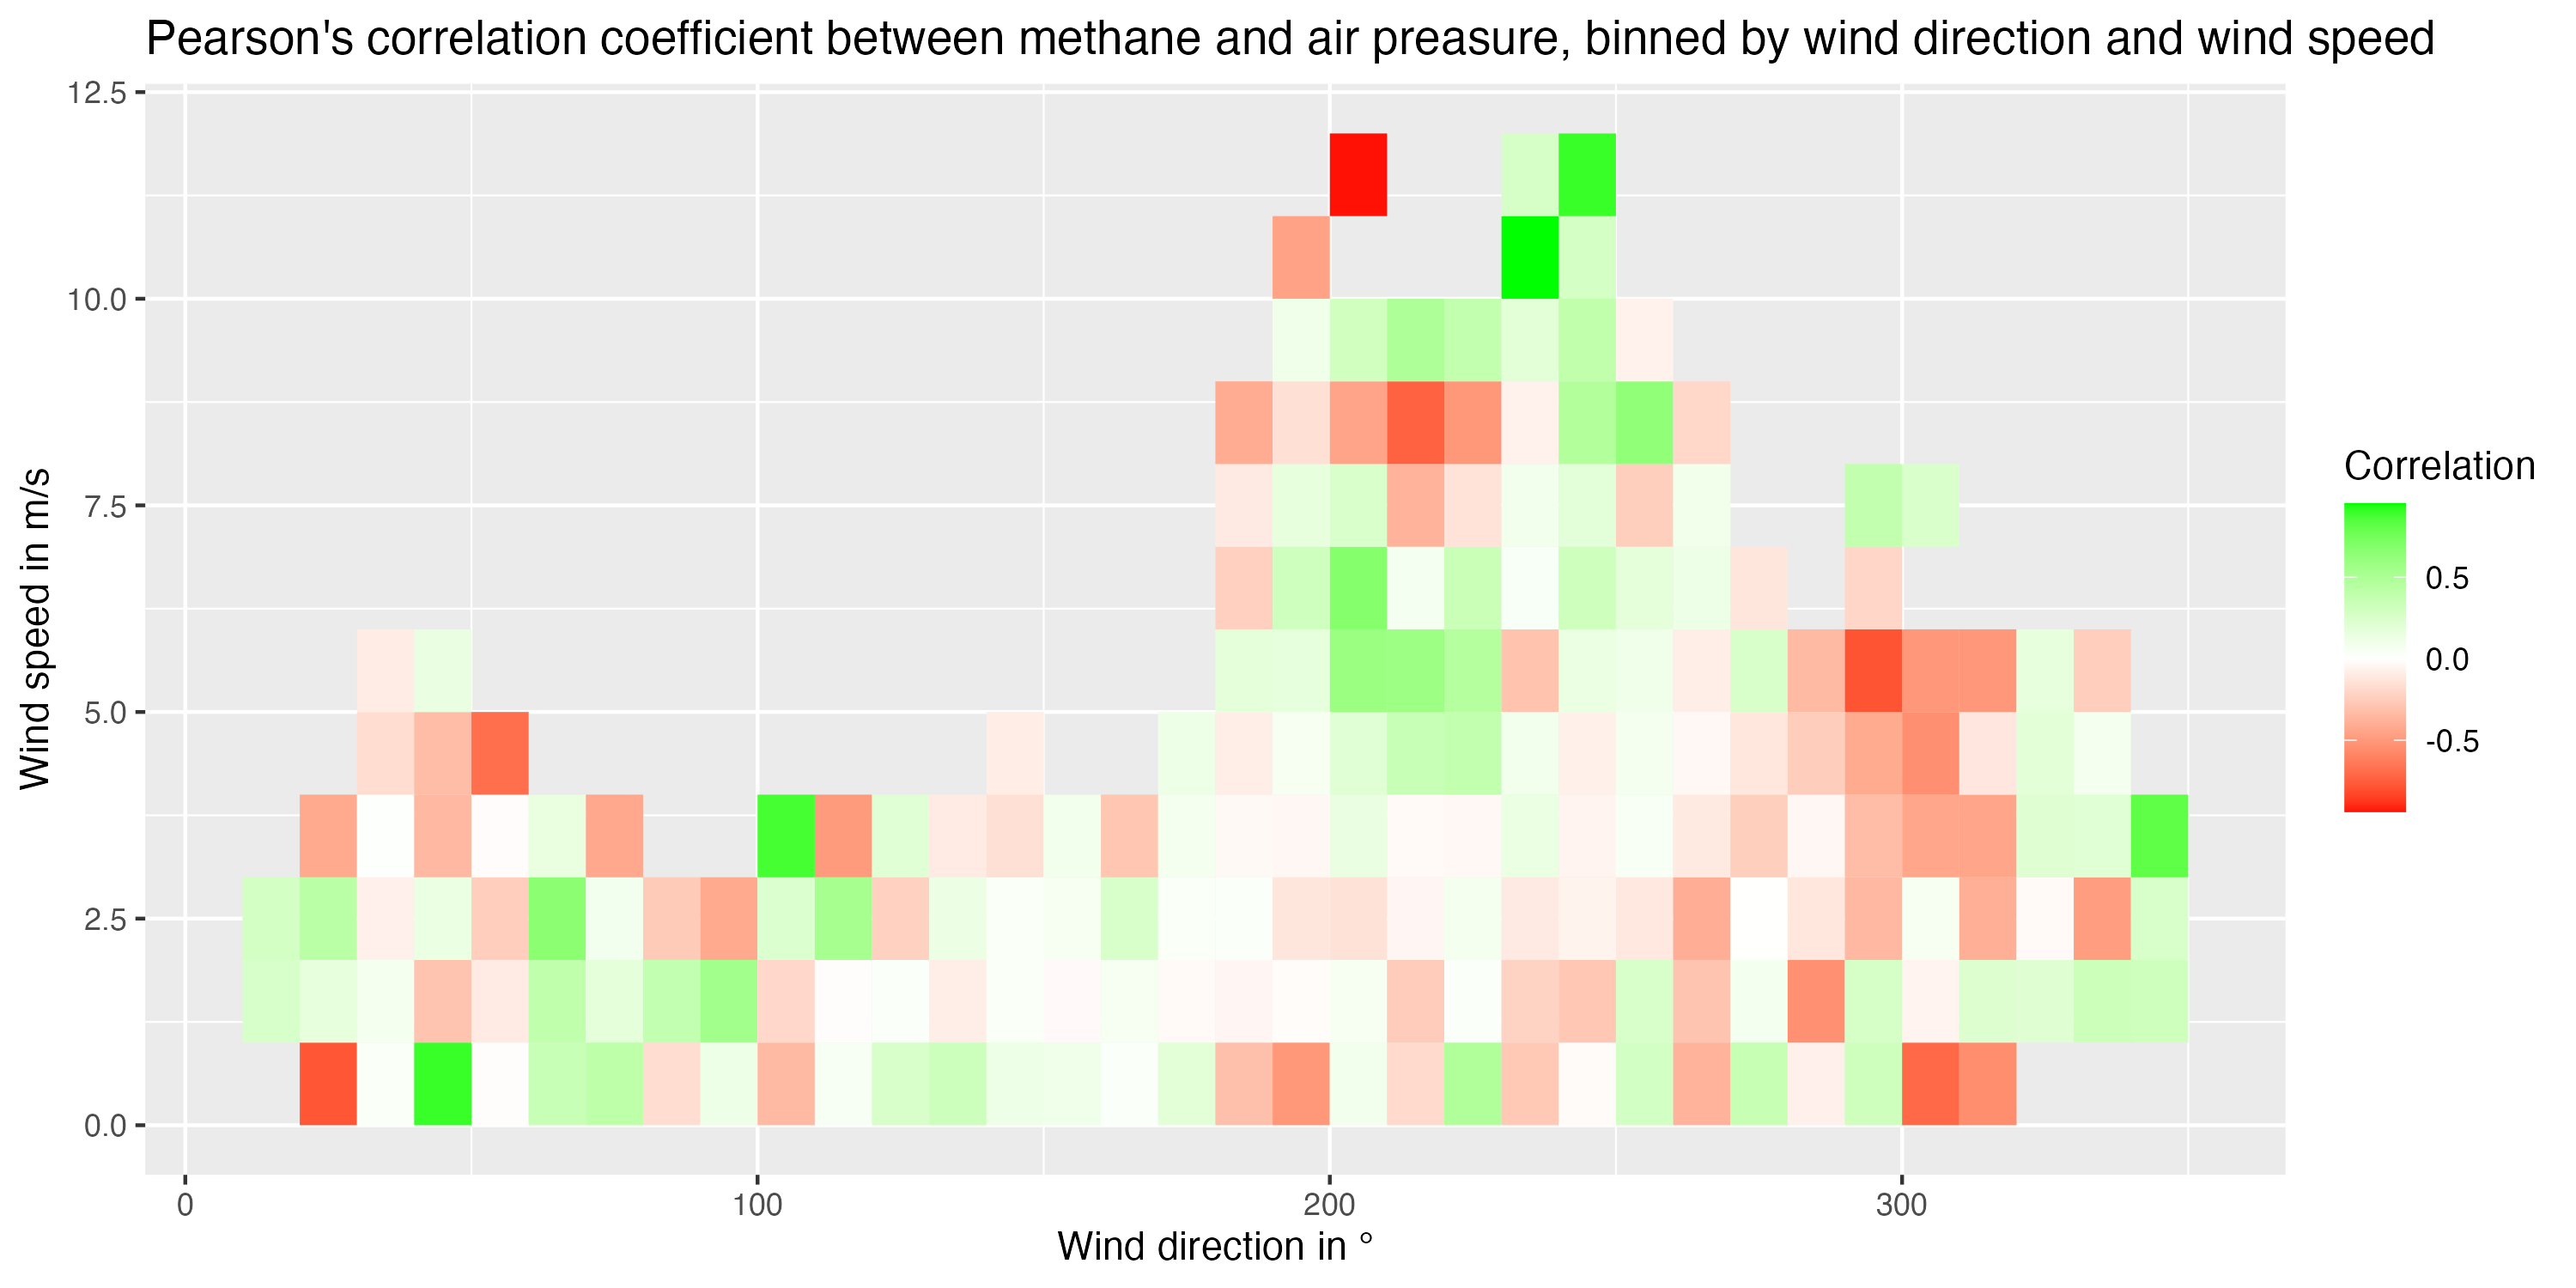
\includegraphics[width=1\linewidth]{figures/Appendix/NoCorrelation/13_CH4_vs_pressure_Correlation_Geomatikum.png}
   \caption[Correlation plot air pressure]{}
   \label{NoCorrelationPressure}
\end{subfigure}
\begin{subfigure}[b]{0.8\textwidth}
   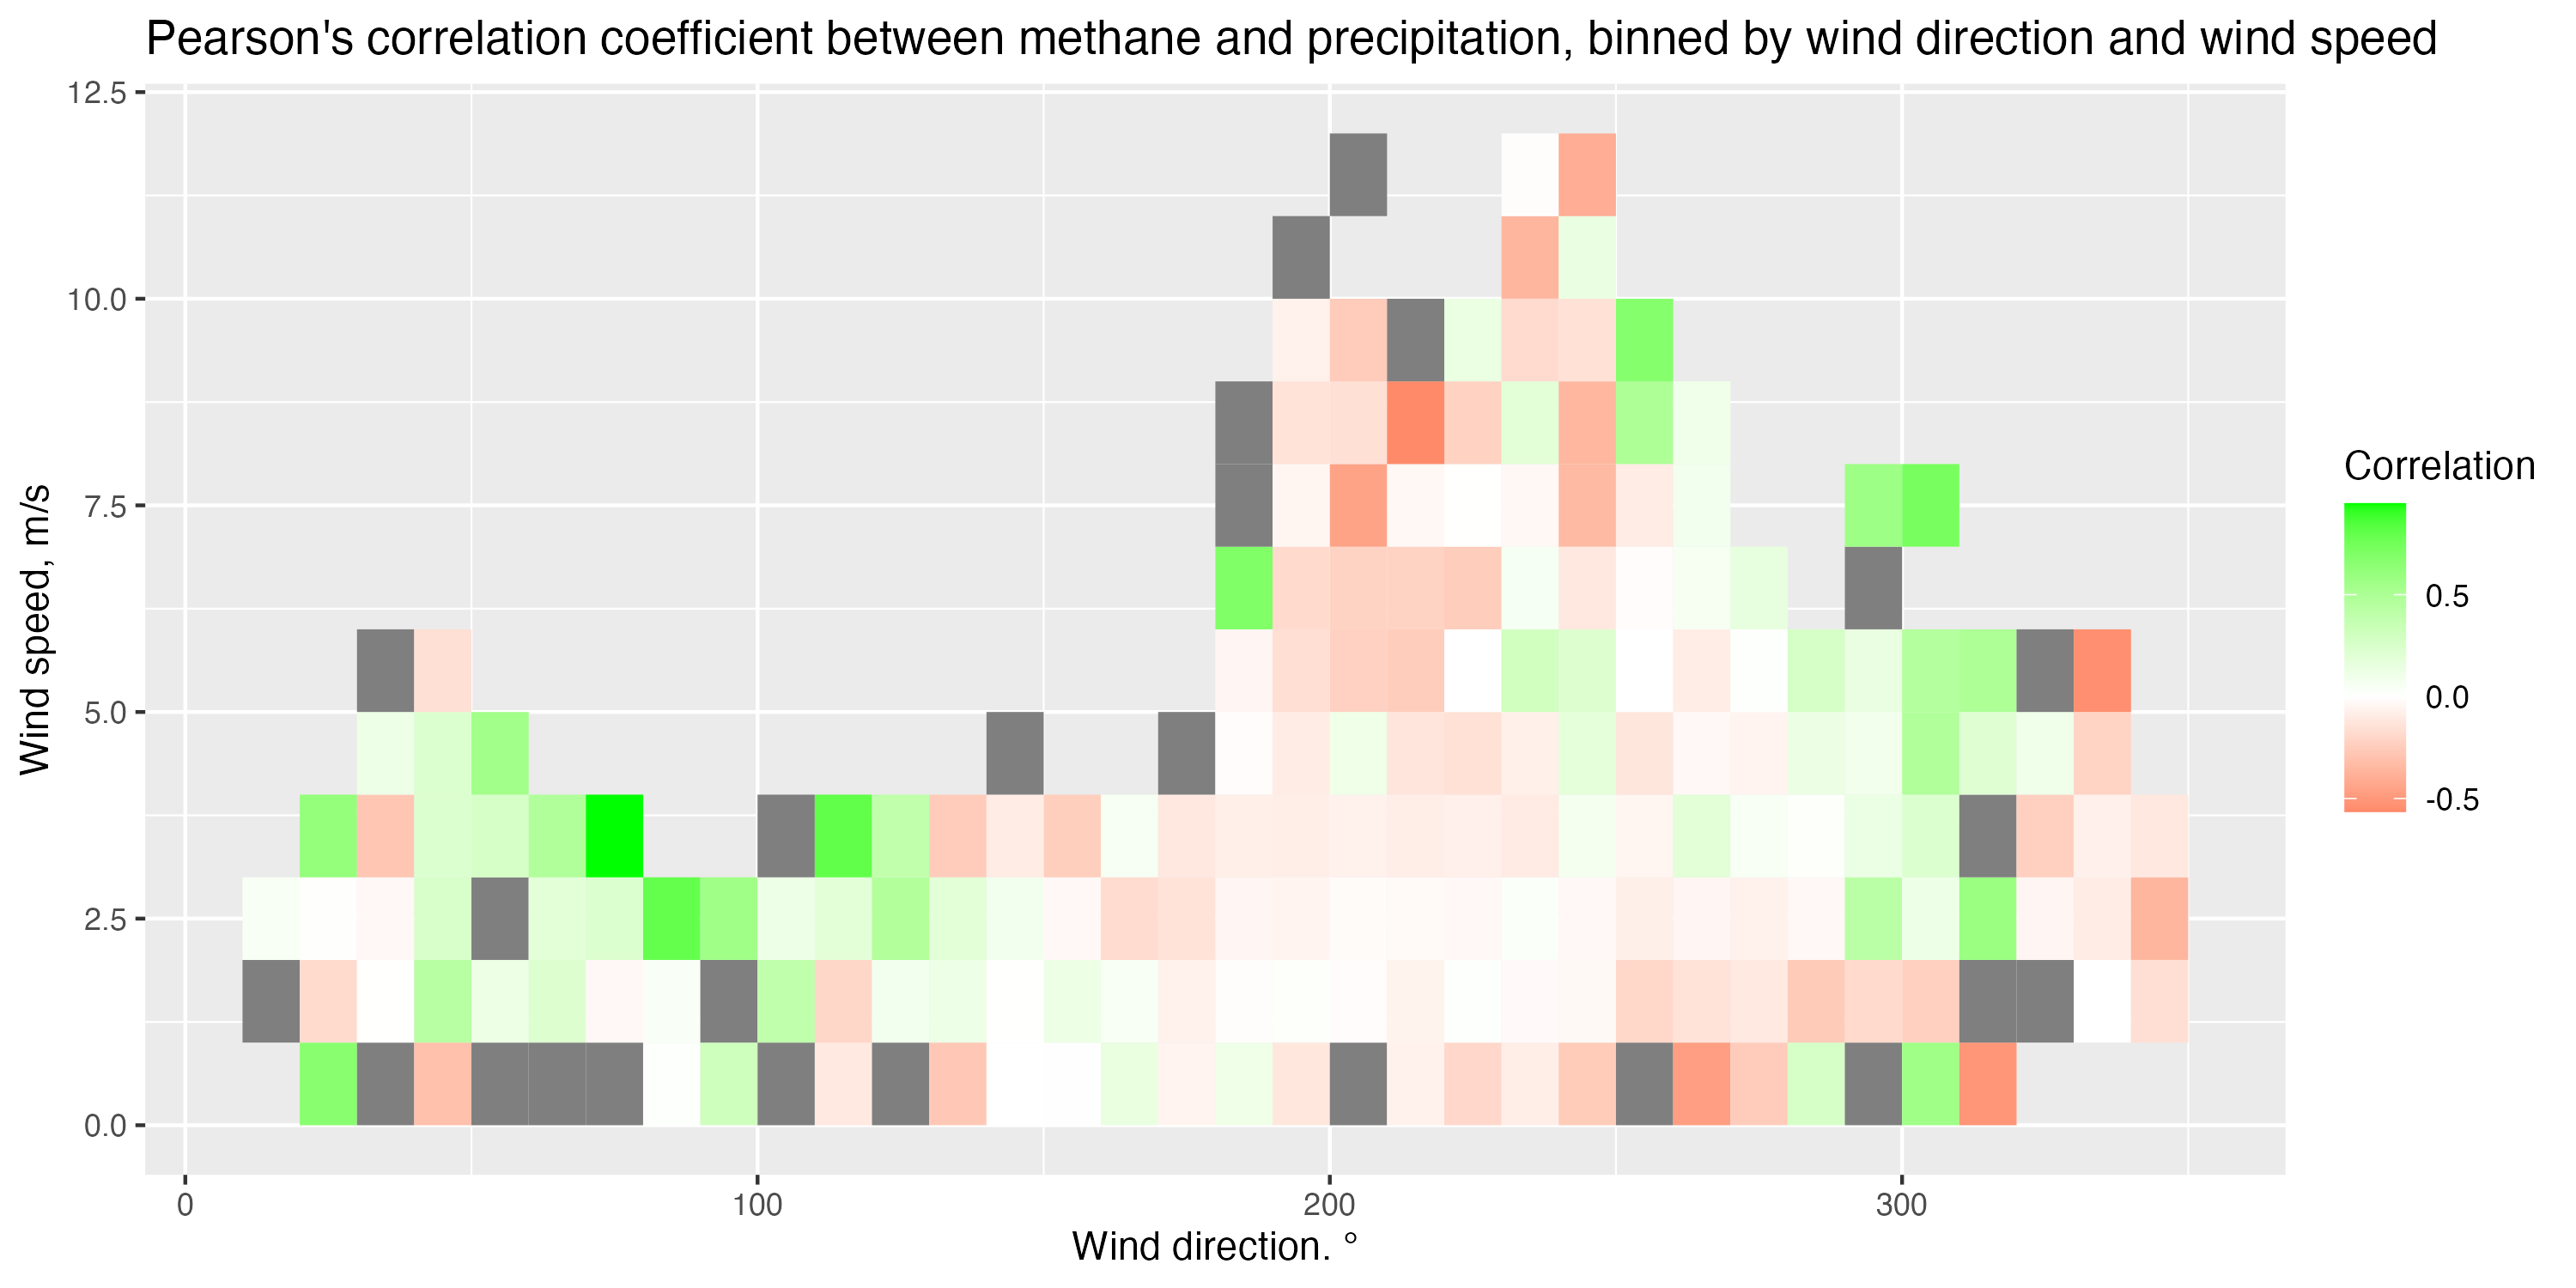
\includegraphics[width=1\linewidth]{figures/Appendix/NoCorrelation/13_CH4_vs_precipitation_height_Correlation_Geomatikum.png}
   \caption[Correlation plot precipitation height]{}
   \label{NoCorrelationPrecipitation}
\end{subfigure}
\caption[Correlation plots showing no correlation with methane concentration in the air]{Pearson's correlation coefficient between methane-air concentration and meteorological/water quality data, binned by wind direction and wind speed. Green shows a positive correlation (enhanced CH$_4$ at high values), and Red shows a negative correlation (enhanced CH$_4$ at low values). (a) Correlation between methane concentration and electrical conductivity in the Elbe water, (b) Correlation betwe(c) Correlation between methane concentration and precipitation height}
\label{NoCorrelationAppendix}
\end{figure}

\begin{figure}[!htb]
\centering
\begin{subfigure}[b]{1\textwidth}
   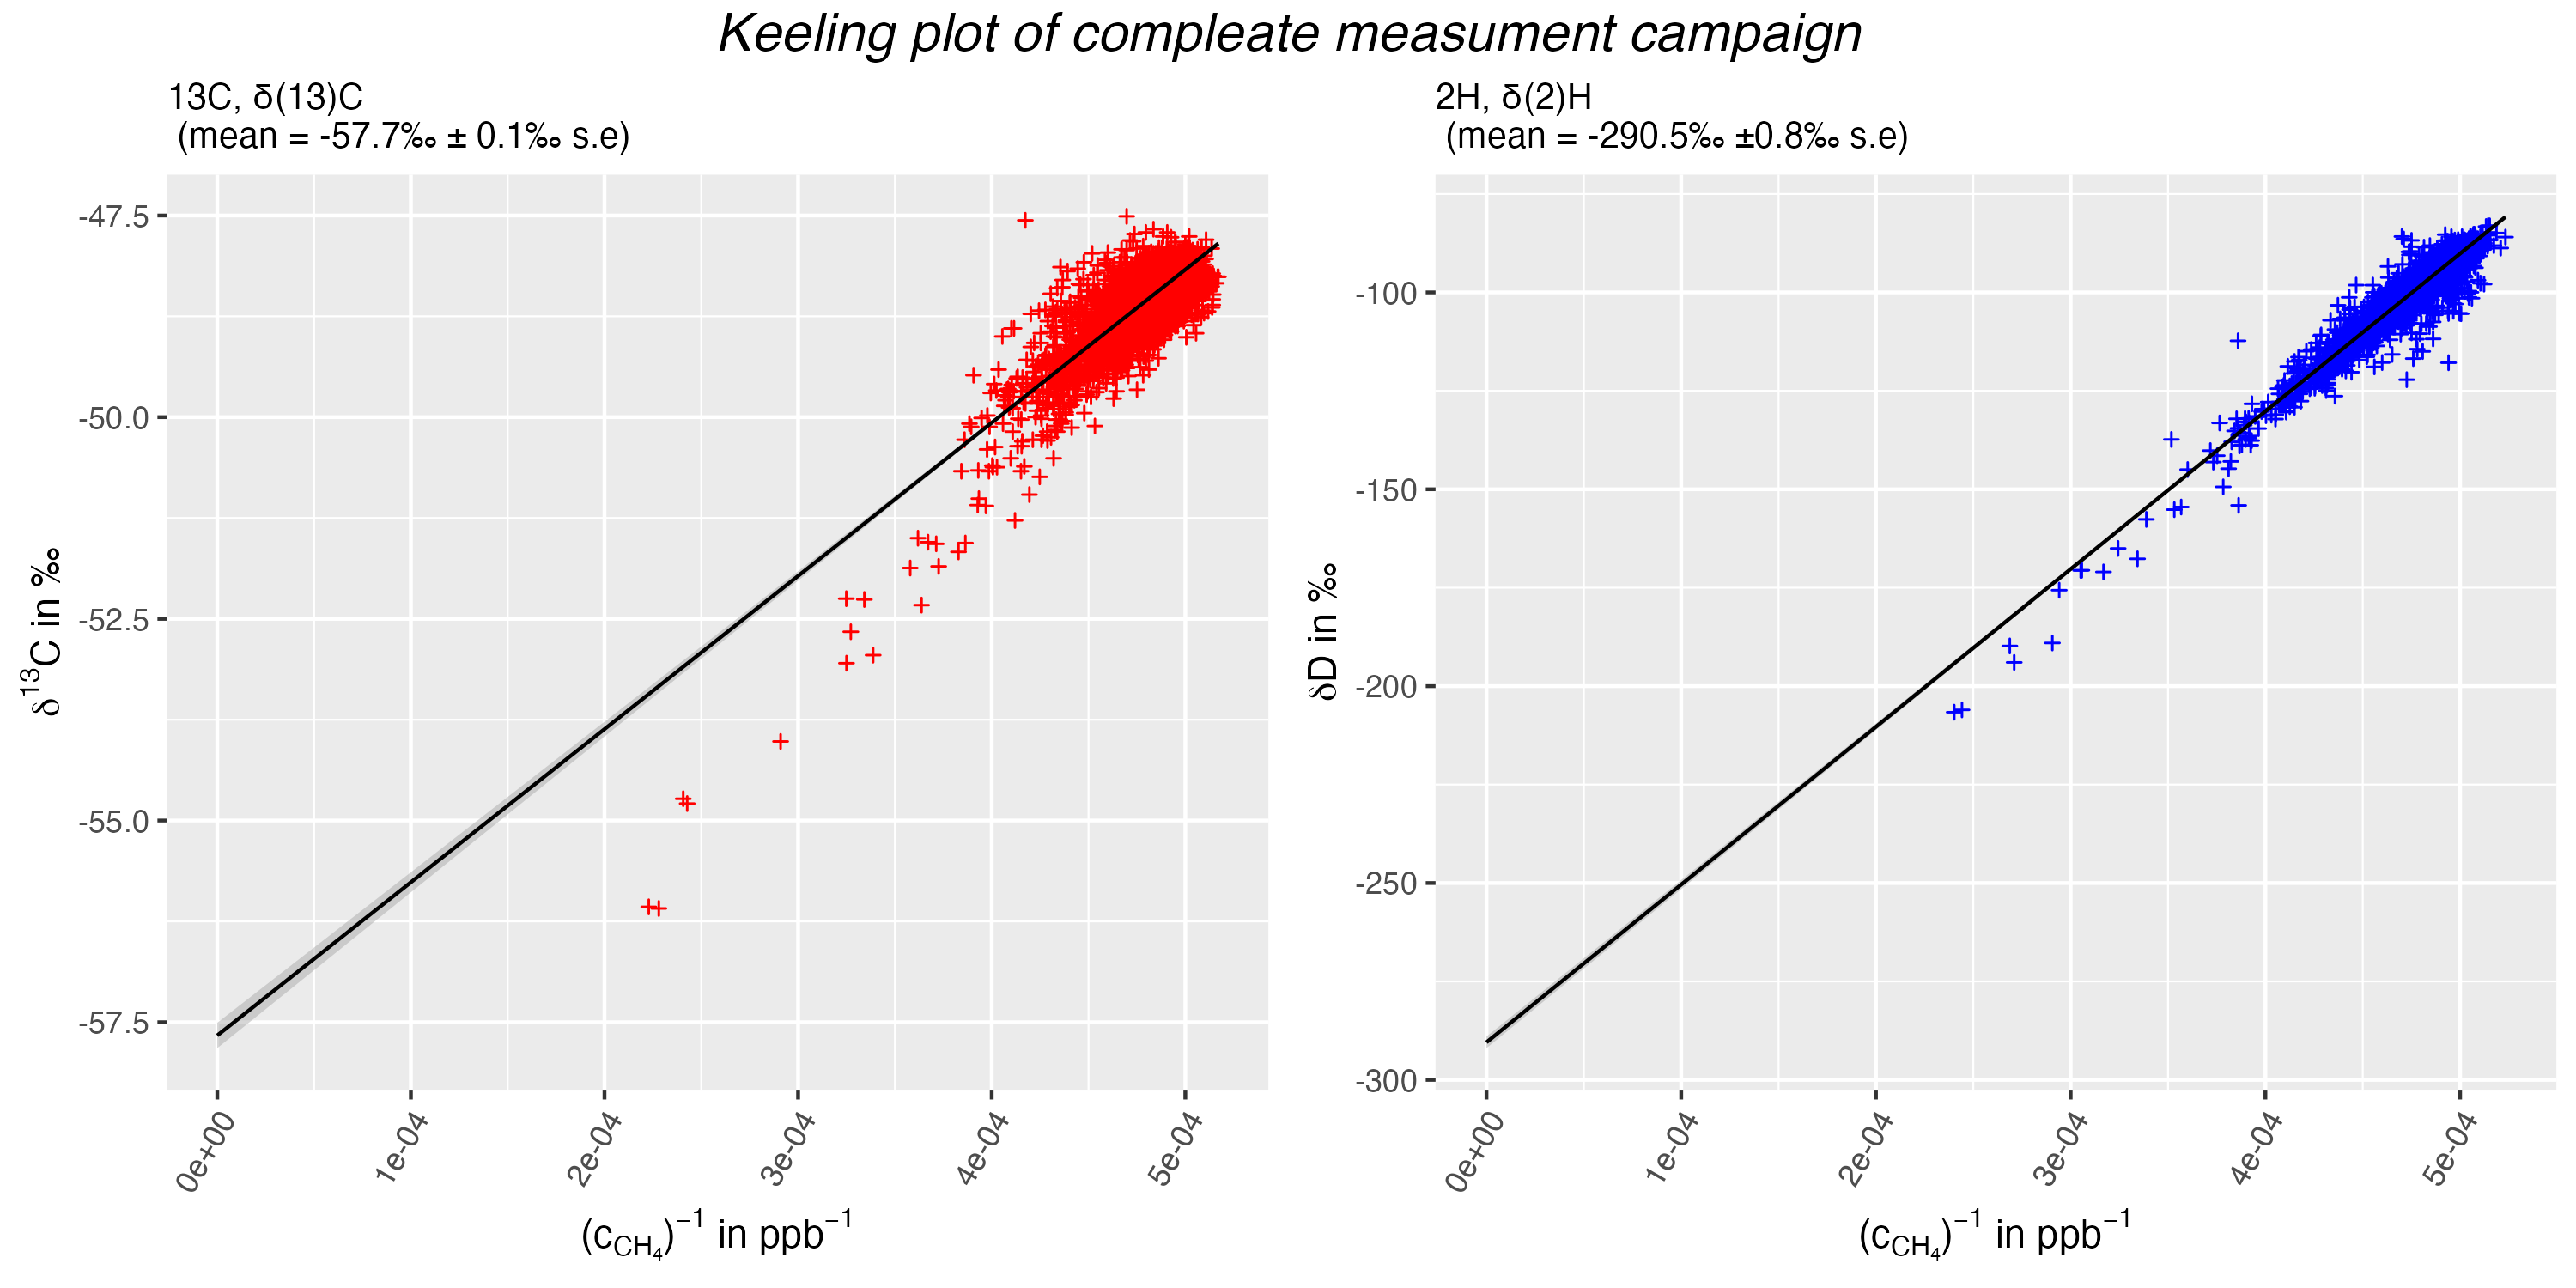
\includegraphics[width=1\linewidth]{figures/Appendix/Keeling/11_Keeling_Plot_Total_paper_peaks.png}
   \caption[Keeling plots total timeline]{}
   \label{KeelingPaperTotal} 
\end{subfigure}

\begin{subfigure}[b]{1\textwidth}
   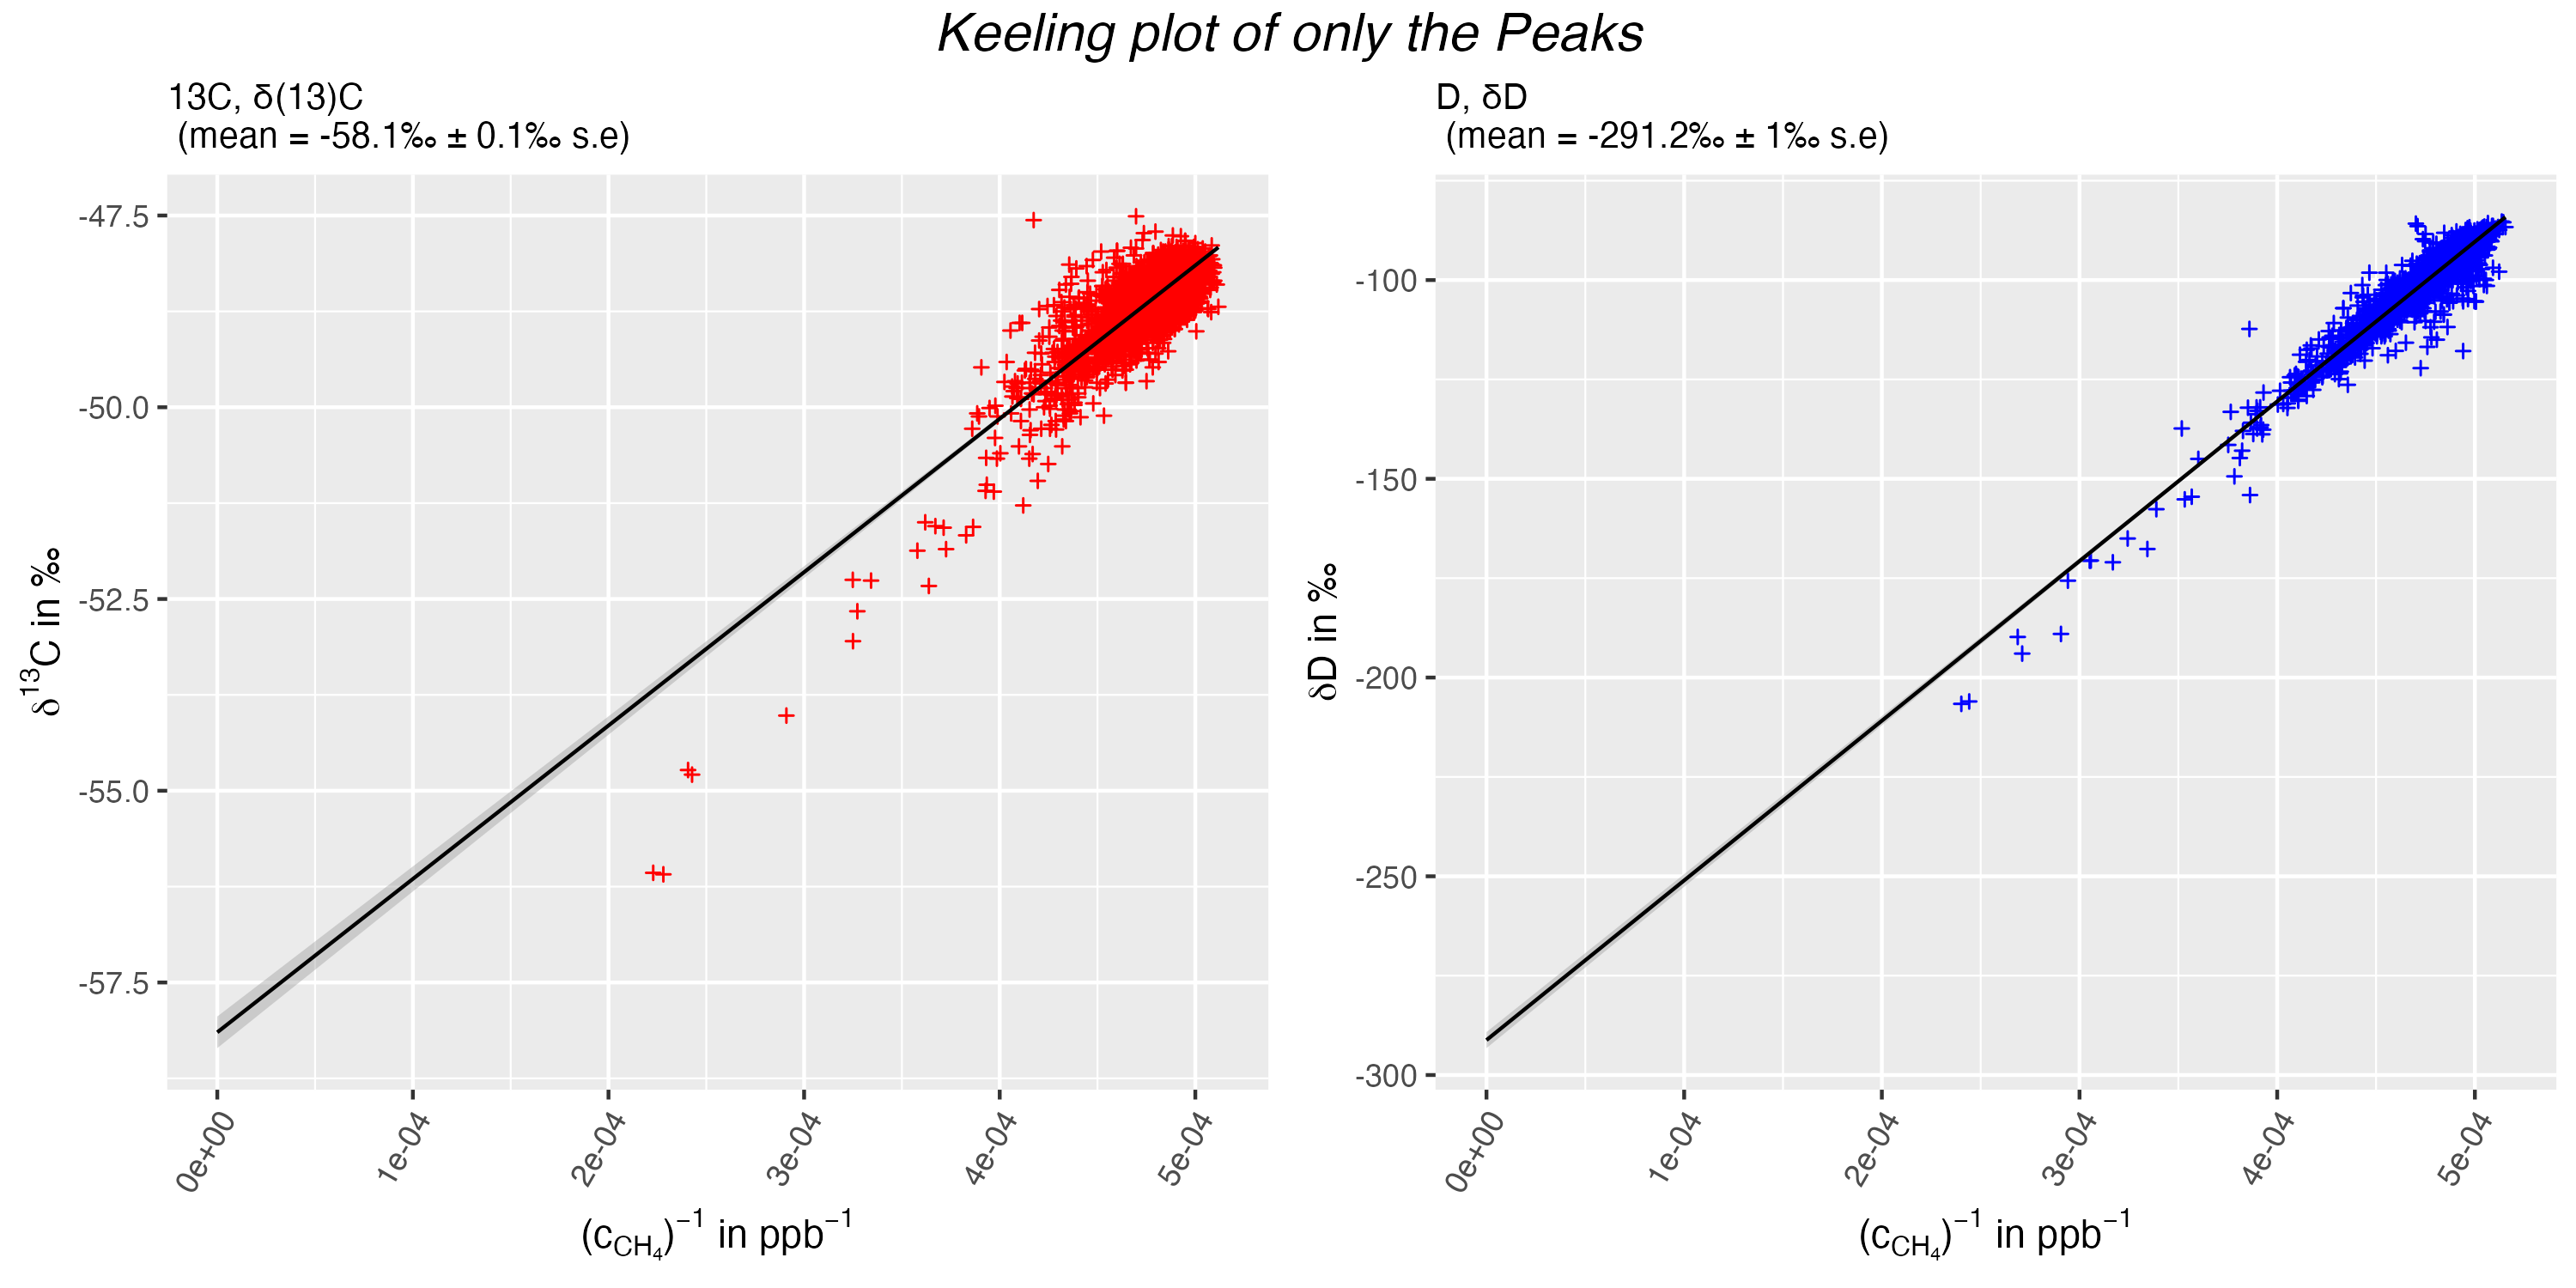
\includegraphics[width=1\linewidth]{figures/Appendix/Keeling/11_Keeling_Plot_Peaks_paper_peaks.png}
   \caption[Keeling plots literature peak identification criteria]{}
   \label{KeelingPaperPeaks}
\end{subfigure}

\caption[Keeling Plot for CH$_4$ peaks in CR-IRMS measurement with peak identification criteria from literature]{Keeling Plots of Carbon-13 and Deuterium in methane peaks measured at the Geomatikum from 1.08.2021 to 1.04.2022. (a) total timeseries with resulting isotopic signatures $\delta$13C = -57.7$\permil$ and $\delta$D = -200.5$\permil$. (b) peak identification criteria by \cite{Menoud.2021}. The resulting isotopic signatures $\delta$13C = -58.1$\permil$ and $\delta$D = -291.2$\permil$}
\label{KeelingPaper}
\end{figure}

\begin{figure}[htbp]
\centering
\begin{subfigure}[b]{1\textwidth}
   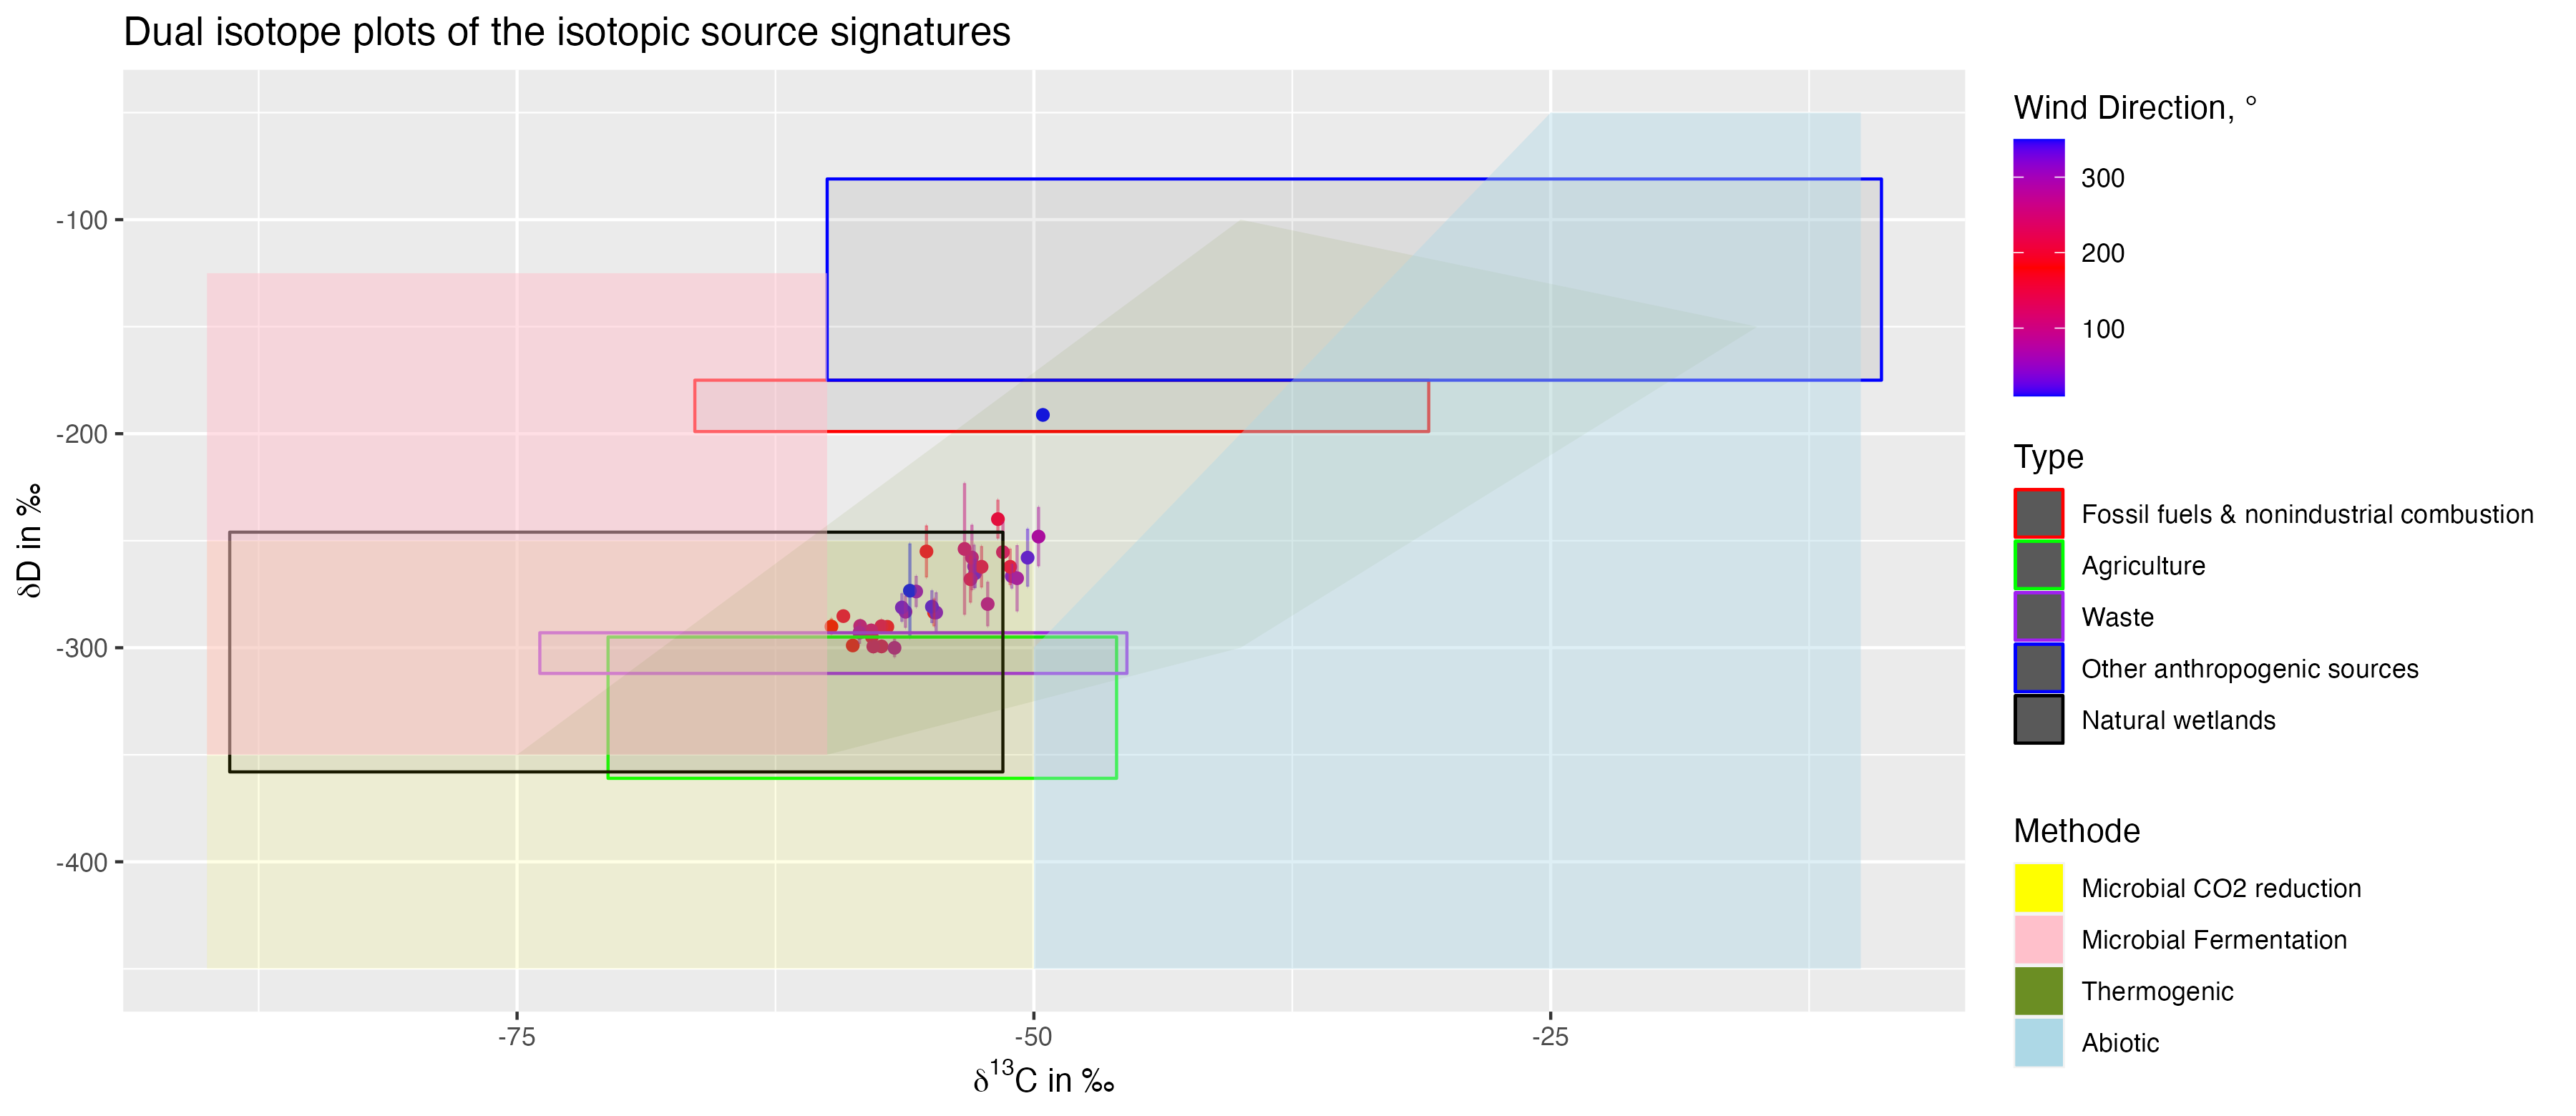
\includegraphics[width=1\linewidth]{figures/Appendix/Keeling/12_Keeling_Total_Wind_paper_peaks.png}
   \caption{}
   \label{DualIsotiotopePaperTotal} 
\end{subfigure}
\begin{subfigure}[b]{1\textwidth}
   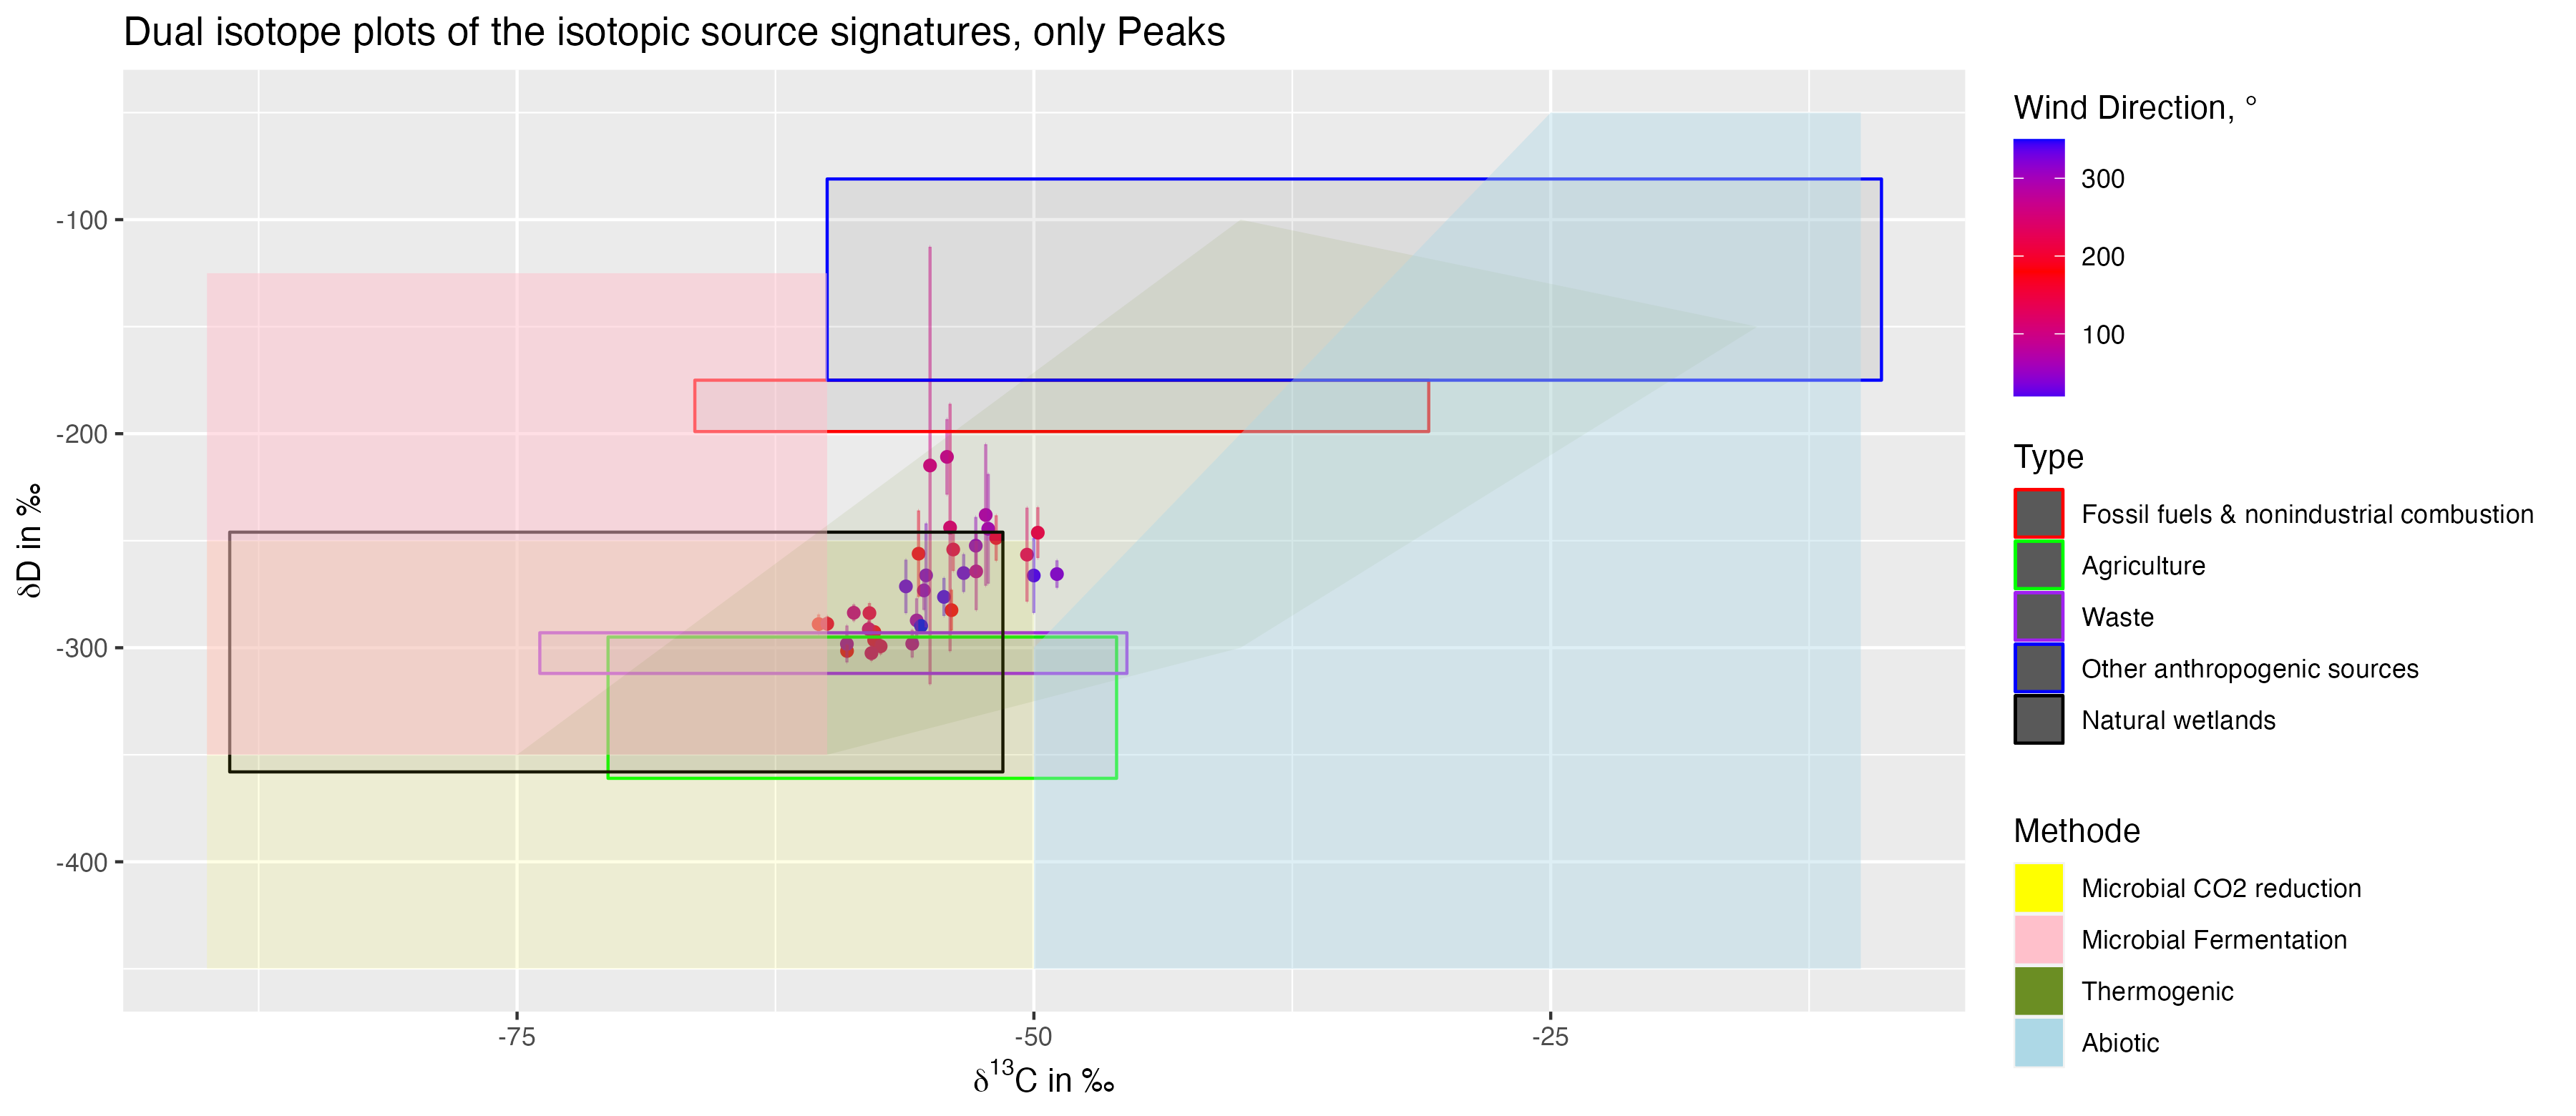
\includegraphics[width=1\linewidth]{figures/Appendix/Keeling/12_Keeling_Peaks_Wind_paper_peaks.png}
   \caption{}
   \label{DualIsotiotopePaperPeaks}
\end{subfigure}
\caption[Dual isotope plot with Literature peak identification criteria]{Dual isotope plot for CF-IRMS measurement for 10° wind direction represented as point colour(blue towards North, red toward South) with highlighted production mechanism (coloured highlight) and source type (coloured boxes). Error bars show one SD. (a) shows total time series, (b) shows only peaks selected with identification criteria by \cite{Menoud.2021}}
\label{DualIsotiotopePlotsAppendix}
\end{figure}

\begin{table}[htbp]
\centering
\begin{tabular}{@{}lllll@{}}
\toprule
W. Direction & $\delta$13C & SE $\delta$13C & $\delta$D & SE $\delta$D \\ \midrule
10        & -49.       & 8.0      & -191      & 2.5     \\
20        & -50.       & 1.9      & -257      & 13.     \\
30        & -52.       & 0.6      & -265      & 6.9     \\
40        & -51.       & 1.0      & -266      & 5.7     \\
50        & -52.       & 0.85     & -261      & 10.     \\
60        & -50.       & 1.1      & -267      & 15.     \\
70        & -49.       & 1.2      & -248      & 13.     \\
80        & -52.       & 0.99     & -279      & 10.     \\
90        & -53.       & 1.3      & -2        & 15.     \\
100       & -53.       & 1.5      & -253      & 30.     \\
110       & -51.       & 1.6      & -255      & 14.     \\
120       & -53.       & 1.2      & -268      & 10.     \\
130       & -52.       & 1.1      & -262      & 9       \\
140       & -51.       & 0.90     & -262      & 8.5     \\
150       & -51.       & 0.9      & -239      & 9.0     \\
160       & -55.       & 0.91     & -255      & 12.     \\
170       & -54        & 0.       & -283      & 6.      \\
180       & -59        & 0.27     & -290      & 3.7     \\
190       & -58.       & 0.23     & -298      & 2.3     \\
200       & -57.       & 0.2      & -290      & 1.9     \\
210       & -59.       & 0.22     & -285      & 2.4     \\
220       & -5         & 0.26     & -294      & 2.0     \\
230       & -57.       & 0.3      & -289      & 3.1     \\
240       & -57.       & 0.32     & -299      & 2.7     \\
250       & -57.       & 0.32     & -299      & 2.8     \\
260       & -57.       & 0.28     & -291      & 2.7     \\
270       & -58        & 0.33     & -289      & 2.8     \\
280       & -56.       & 0.51     & -30       & 4.3     \\
290       & -58.       & 0.43     & -29       & 5.2     \\
300       & -56.       & 0.68     & -283      & 7.5     \\
310       & -55.       & 0.96     & -273      & 7.2     \\
320       & -54.       & 0.75     & -283      & 9.4     \\
330       & -56.       & 0.74     & -281      & 6.6     \\
340       & -54.       & 1.0      & -28       & 7.6     \\
350       & -55.       & 3.2      & -273      & 22.     \\ \bottomrule
\end{tabular}
\label{WindKeelingTableTotalAppendix}
\caption[Windrose by DWD and Universität Hamburg]{Table of isotopc signature of $\delta$13C and $\delta$D by Keeling analyse for the total CF-IRMS measurement at the Geomatikum, 01.08.2022 to 01.03.2022, separated in wind directions during the measurement.}
\end{table}


\begin{figure}\centering
\subfloat[]{\label{WindRoseDWD}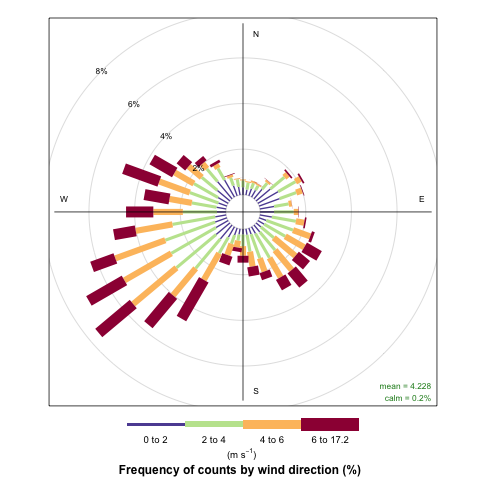
\includegraphics[width=.45\linewidth]{figures/Appendix/Windrose/WindRose_Total_DWD.png}}\hfill
\subfloat[]{\label{WindRose50m}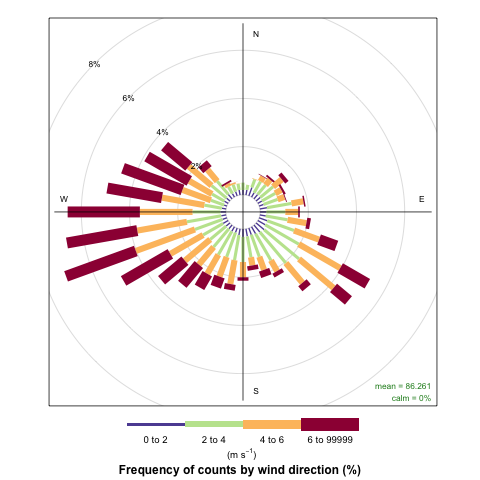
\includegraphics[width=.45\linewidth]{figures/Appendix/Windrose/WindRose_Total_50m.png}}\par 
\subfloat[]{\label{WindRose110m}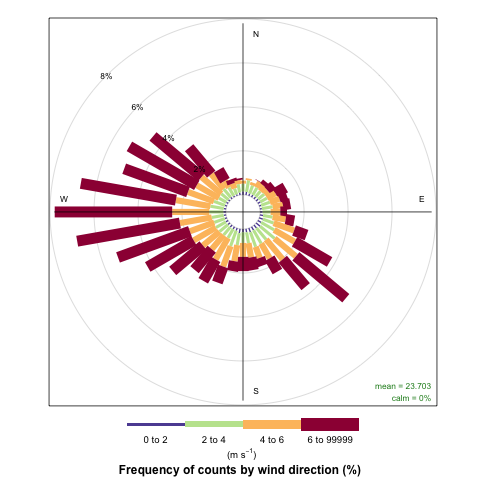
\includegraphics[width=.45\linewidth]{figures/Appendix/Windrose/WindRose_Total_110m.png}}
\caption[Windrose by DWD and Universität Hamburg]{Windrose plots with data from (a) Deutscher Wetterdienst (DWD) (\cite{DeutschenWetterdienst.20230501}) at Fuhlsbüttel, Hamburg and Universität Hamburg \cite{Lange.20220501} with wind measurements at (b) 50 m and (c) 110m}
\label{WindRoseAppendix}
\end{figure}




\begin{figure}[htbp]
 \centering
 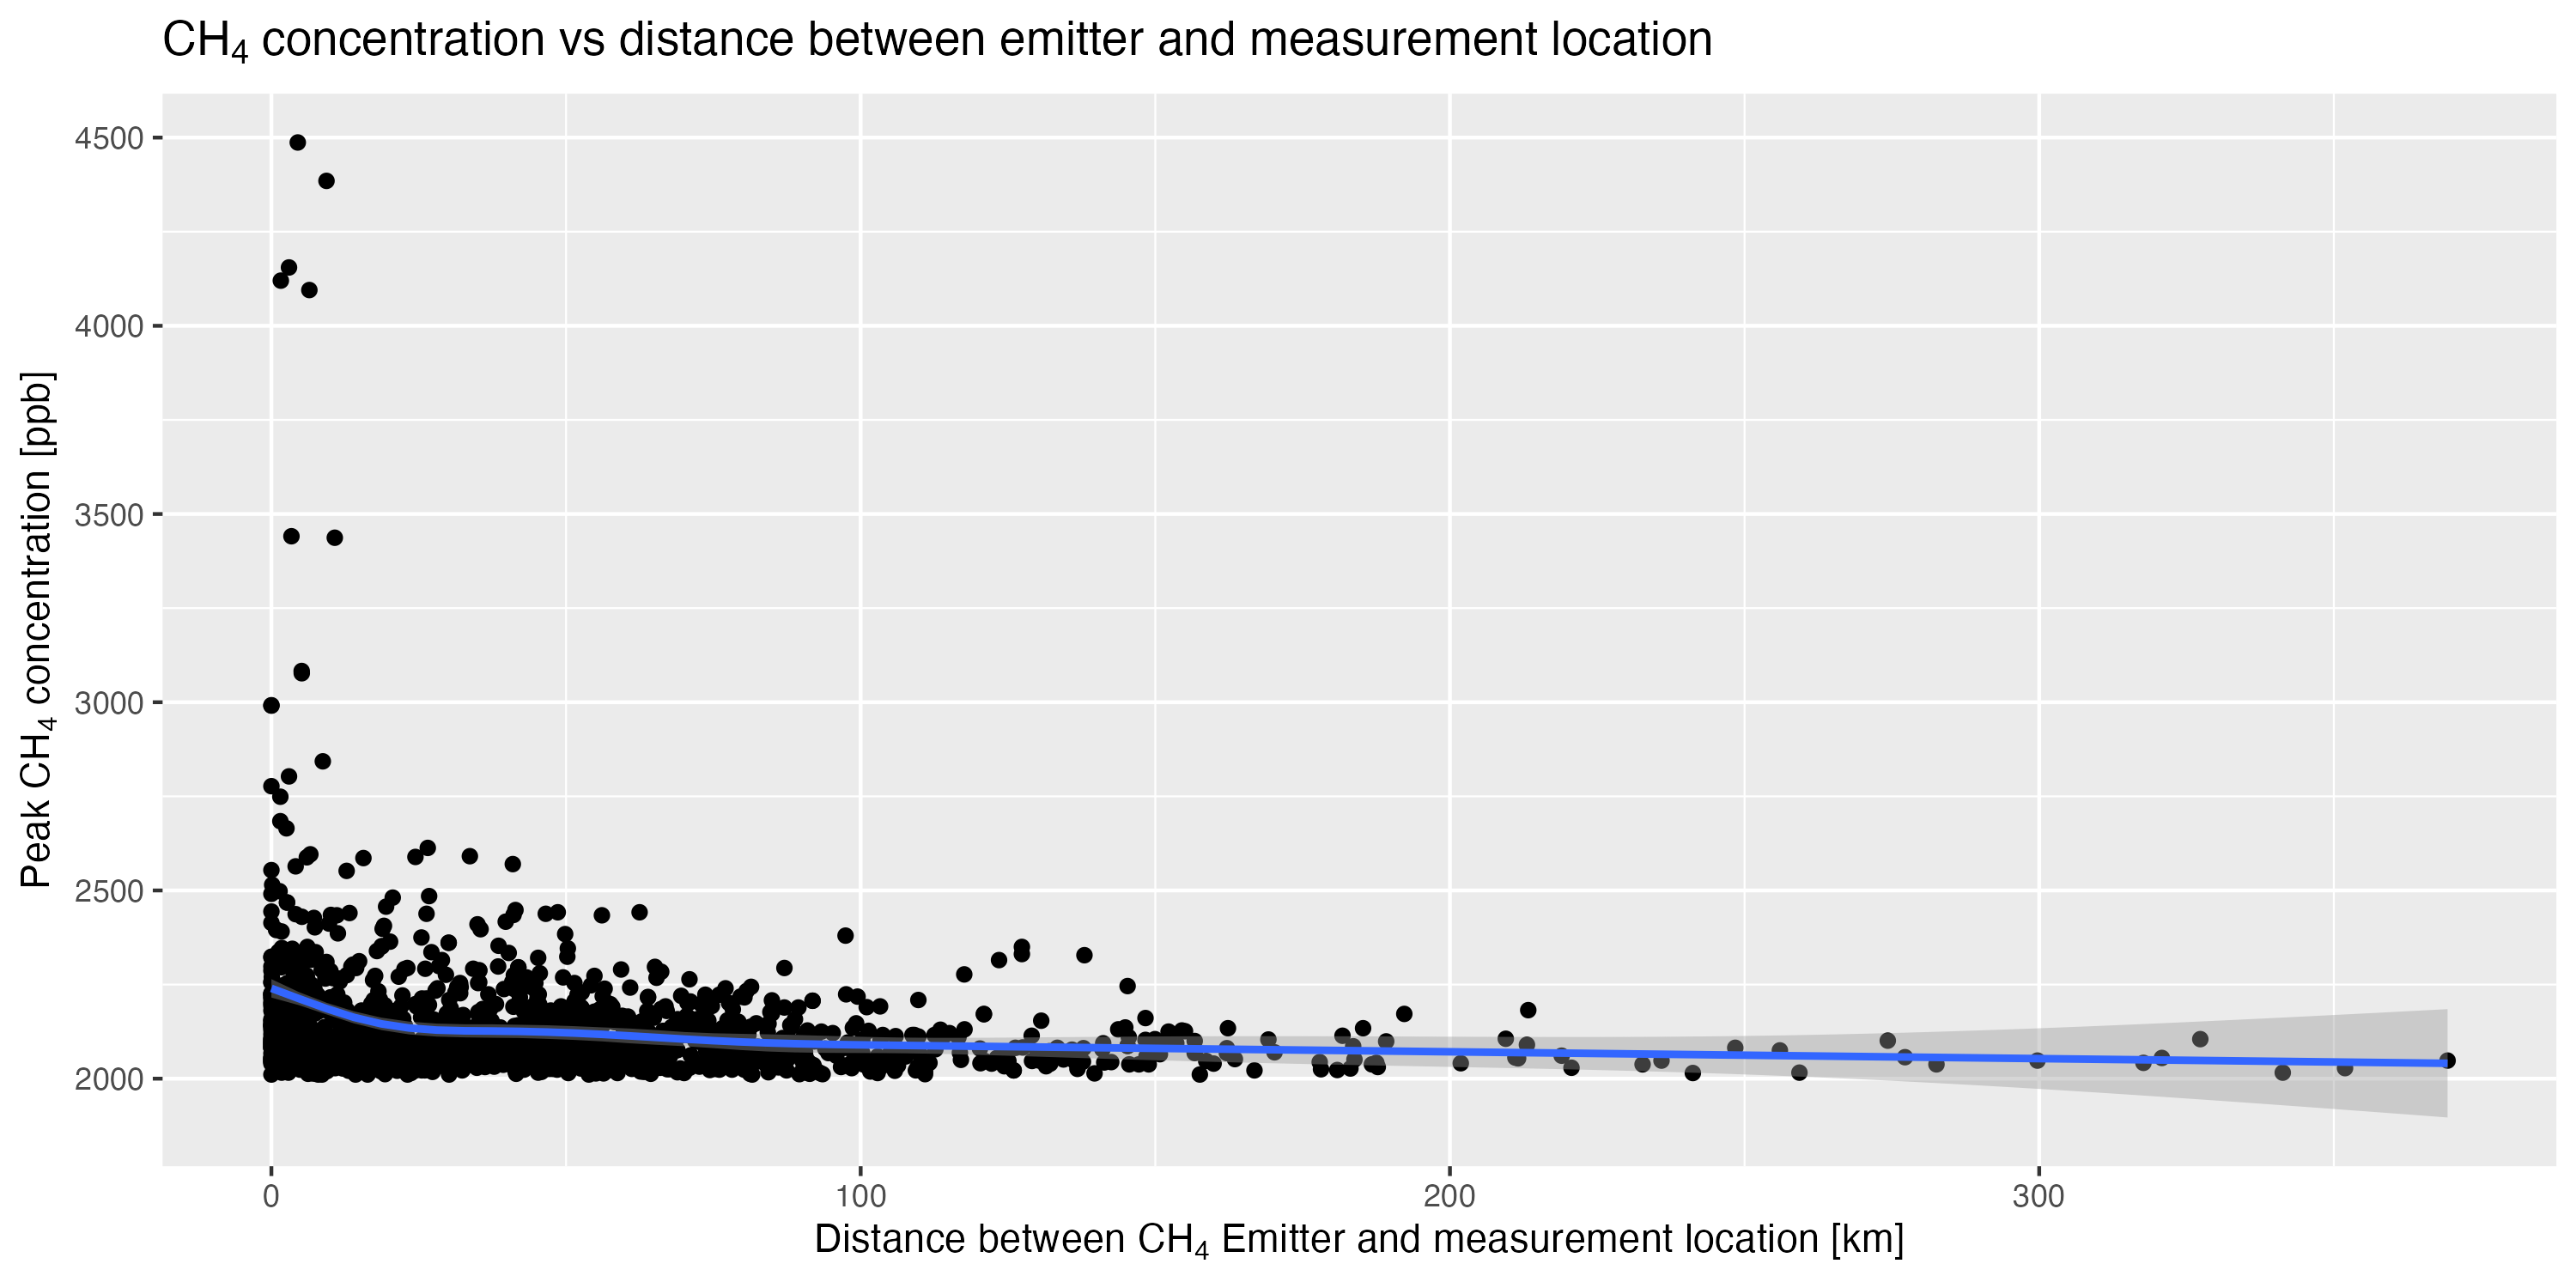
\includegraphics[width=1\textwidth]{figures/Appendix/Transportmodel/14_Low_WL_to_Peak_distance_paper_peaks.png}
 \caption[Distance between estimated emitter and measurement location]{Scatter plot of modelled Distance between the estimated emission location and the measurement location at the Geomatikum, against the methane concentration observed at the Geomatikum measured by the CF-IRMS. A local regression line is fitted to the plot (Blue). The standard error of the line is shown in dark grey. The peaks were identified using the identification criteria by \cite{Menoud.2021}}
 \label{DistancePlotPaperAppendix}
\end{figure}

\begin{figure}[htbp]
\centering
\begin{subfigure}[b]{1\textwidth}
   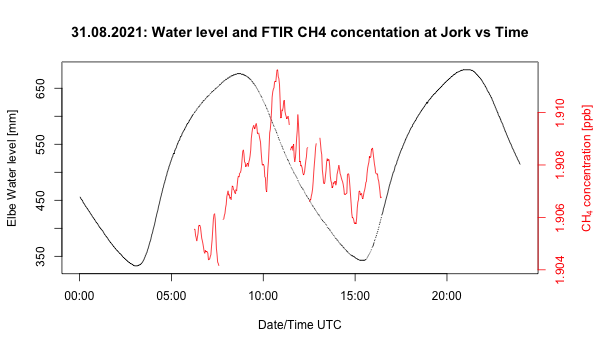
\includegraphics[width=1\linewidth]{figures/Appendix/FTIR/15_Basic_Plot_CH4_Wl_FTIR202108031mc.png}
   \caption{}
   \label{FTIRWLJork} 
\end{subfigure}
\begin{subfigure}[b]{1\textwidth}
   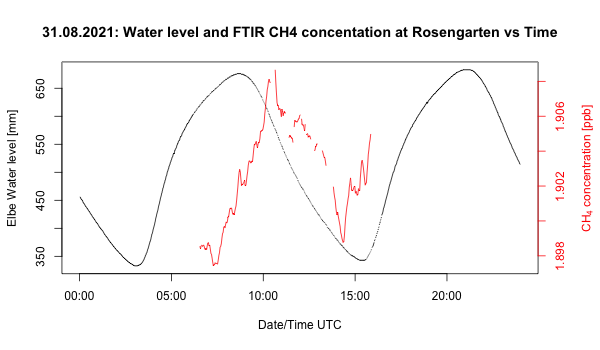
\includegraphics[width=1\linewidth]{figures/Appendix/FTIR/15_Basic_Plot_CH4_Wl_FTIR202108031md.png}
   \caption{}
   \label{FTIRWLRosengarten}
\end{subfigure}
\caption[FTIR with water level overlay timeline]{Plot of the total column methane concentration measured (Red line) overlayed with the Elbe water level measured at St.
Pauli (Black line). The measurements were performed on 31.08.2021. (a) measured at Jork, (b) measured at Rosengarten. A low water methane peak can be seen at 16:00 UTC.}
\label{FTIRWLAppendix}
\end{figure}